%%%%% Set up %%%%%

% Set document style and font size
\documentclass[12pt]{article}\usepackage[]{graphicx}\usepackage[]{color}
%% maxwidth is the original width if it is less than linewidth
%% otherwise use linewidth (to make sure the graphics do not exceed the margin)
\makeatletter
\def\maxwidth{ %
  \ifdim\Gin@nat@width>\linewidth
    \linewidth
  \else
    \Gin@nat@width
  \fi
}
\makeatother

\definecolor{fgcolor}{rgb}{0.345, 0.345, 0.345}
\newcommand{\hlnum}[1]{\textcolor[rgb]{0.686,0.059,0.569}{#1}}%
\newcommand{\hlstr}[1]{\textcolor[rgb]{0.192,0.494,0.8}{#1}}%
\newcommand{\hlcom}[1]{\textcolor[rgb]{0.678,0.584,0.686}{\textit{#1}}}%
\newcommand{\hlopt}[1]{\textcolor[rgb]{0,0,0}{#1}}%
\newcommand{\hlstd}[1]{\textcolor[rgb]{0.345,0.345,0.345}{#1}}%
\newcommand{\hlkwa}[1]{\textcolor[rgb]{0.161,0.373,0.58}{\textbf{#1}}}%
\newcommand{\hlkwb}[1]{\textcolor[rgb]{0.69,0.353,0.396}{#1}}%
\newcommand{\hlkwc}[1]{\textcolor[rgb]{0.333,0.667,0.333}{#1}}%
\newcommand{\hlkwd}[1]{\textcolor[rgb]{0.737,0.353,0.396}{\textbf{#1}}}%
\let\hlipl\hlkwb

\usepackage{framed}
\makeatletter
\newenvironment{kframe}{%
 \def\at@end@of@kframe{}%
 \ifinner\ifhmode%
  \def\at@end@of@kframe{\end{minipage}}%
  \begin{minipage}{\columnwidth}%
 \fi\fi%
 \def\FrameCommand##1{\hskip\@totalleftmargin \hskip-\fboxsep
 \colorbox{shadecolor}{##1}\hskip-\fboxsep
     % There is no \\@totalrightmargin, so:
     \hskip-\linewidth \hskip-\@totalleftmargin \hskip\columnwidth}%
 \MakeFramed {\advance\hsize-\width
   \@totalleftmargin\z@ \linewidth\hsize
   \@setminipage}}%
 {\par\unskip\endMakeFramed%
 \at@end@of@kframe}
\makeatother

\definecolor{shadecolor}{rgb}{.97, .97, .97}
\definecolor{messagecolor}{rgb}{0, 0, 0}
\definecolor{warningcolor}{rgb}{1, 0, 1}
\definecolor{errorcolor}{rgb}{1, 0, 0}
\newenvironment{knitrout}{}{} % an empty environment to be redefined in TeX

\usepackage{alltt}

% File path to resources (style file etc)
\newcommand{\locRepo}{csas-style}

% Style file for DFO Technical Reports
\usepackage{\locRepo/tech-report}

% header-includes from R markdown entry
\usepackage{float}

%%%%% Variables %%%%%

% New definitions: Title, year, report number, authors
% Protect lower case words (i.e., species names) in \Addlcwords{}, in "TechReport.sty"
\newcommand{\trTitle}{Development of methods in support of a head-only sampling program for Sablefish (\emph{Anoplopoma fimbria}) in British Columbia}
\newcommand{\trYear}{2023}
\newcommand{\trReportNum}{nnn}
% Optional
\newcommand{\trAuthFootA}{Email: \link{mailto:Lacko.Lisa@dfo-mpo.gc.ca}{\nolinkurl{Lacko.Lisa@dfo-mpo.gc.ca}} \textbar{} telephone: (778) 268-3236}
\newcommand{\trAuthsLong}{Lisa. C. Lacko\textsuperscript{1} and Kathryn L. Temple\textsuperscript{1} and Kendra R. Holt\textsuperscript{1} and Janine K. Supernault\textsuperscript{1} and Kronlund, A. R.\textsuperscript{2} and Malcolm R. Wyeth\textsuperscript{1} and Brendan M. Conners\textsuperscript{1}}
\newcommand{\trAuthsBack}{Lacko, L.C., Temple, K.L., Holt, K.R., Supernault, J.K.,Kronlund, A.R., Wyeth, M.R, and Conners, B.M.}

% New definition: Address
\newcommand{\trAddy}{\textsuperscript{1}Pacific Biological Station\\
Fisheries and Oceans Canada, 3190 Hammond Bay Road\\
Nanaimo, British Columbia, V9T 6N7, Canada\\
\strut \\
\textsuperscript{2}Interface Fisheries Consulting, Ltd.\\
Unit 30, 4300 Stoneywood Lane,\\
Victoria, British Columbia, V8X 5A5\\}

% Abstract
\newcommand{\trAbstract}{Routine biological sampling of whole round Sablefish from commercial fishing operations in British Columbia began the early 1990's. Historically, round specimens were obtained through voluntary commercial fishery catch sampling and tag recovery programs. We investigate the potential for obtaining sex and length information using heads, rather than the entire fish to promote participation in the sampling programs. In 2016, 438 Sablefish (240-1080 mm) were sampled at sea and six different fish head measurements were collected. Genetic samples (137) were obtained to develop methods of DNA-based sex identification. Regression analysis results reveal that all six cranial dimensions can be used to accurately predict length. However, interorbital distance was not only a good predictor of length, but samplers ranked it the most efficient to measure and easily repeatable. A pilot study occurred in 2017 with 360 head-only samples collected and sexed by a commercial vessel, followed by scientific sampling on shore. Genomic DNA were successfully processed for 80 of 99 samples. Fisher sex determination was accurate 84\% of the time. Given the results, the 2018 commercial sampling collection program was modified so that returns of whole round Sablefish were replaced by head-only samples with knife cuts on the operculum to indicate sex.}

% Resume (i.e., French abstract)
\newcommand{\trResume}{L'échantillonnage biologique périodique de morues charbonnières entières provenant des activités de pêche commerciale en Colombie-Britannique a commencé au début des années 1990. Historiquement, des spécimens entiers ont été recueillis dans le cadre de programmes volontaires d'échantillonnage des prises commerciales et de récupération d'étiquettes. Nous étudions la possibilité d'obtenir de l'information sur le sexe et la longueur en utilisant les têtes seulement plutôt que les poissons entiers afin de favoriser la participation aux programmes d'échantillonnage. En 2016, 438 morues charbonnières (de 240 à 1 080 mm) ont été échantillonnées en mer et six différentes mesures de la tête des poissons ont été recueillies. Des échantillons génétiques (137) ont été obtenus afin de mettre au point des méthodes de sexage fondées sur l'ADN. Les résultats de l'analyse de régression révèlent que les six mesures de la dimension du crâne peuvent toutes permettre de prédire la longueur avec précision. Cependant, la distance interorbitale s'est non seulement révélée un bon prédicteur de la longueur, mais les échantillonneurs ont aussi déterminé qu'il s'agissait de la mesure la plus efficace et la plus facilement répétable. Une étude pilote a été menée en 2017, au cours de laquelle 360 échantillons de tête seulement ont été obtenus et sexés en mer à bord d'un bateau de pêche commercial, puis échantillonnés à terre par une équipe scientifique. L'ADN génomique de 80 échantillons sur 99 a été traité avec succès. La détermination du sexe par les pêcheurs était exacte 84 \% du temps. Compte tenu de ces résultats, le programme d'échantillonnage des prises commerciales de 2018 a été modifié de sorte que les échantillons retournés ne sont plus des morues charbonnières entières, mais seulement des têtes avec une entaille au couteau sur l'opercule indiquant le sexe.}

\newcommand{\trISBN}{}

\DeclareGraphicsExtensions{.png,.pdf}
%%%%% Start %%%%%

% Start the document
\IfFileExists{upquote.sty}{\usepackage{upquote}}{}

% commands and environments needed by pandoc snippets
% extracted from the output of `pandoc -s`
%% Make R markdown code chunks work
\usepackage{array}
\usepackage{amssymb,amsmath}
\usepackage{color}
\usepackage{fancyvrb}

% From default template:
\newcommand{\VerbBar}{|}
\newcommand{\VERB}{\Verb[commandchars=\\\{\}]}
\DefineVerbatimEnvironment{Highlighting}{Verbatim}{commandchars=\\\{\},formatcom=\color[rgb]{0.00,0.00,0.00}}
\usepackage{framed}
\definecolor{shadecolor}{RGB}{248,248,248}
\newenvironment{Shaded}{\begin{snugshade}}{\end{snugshade}}
\newcommand{\AlertTok}[1]{\textcolor[rgb]{0.94,0.16,0.16}{#1}}
\newcommand{\AnnotationTok}[1]{\textcolor[rgb]{0.56,0.35,0.01}{\textbf{\textit{#1}}}}
\newcommand{\AttributeTok}[1]{\textcolor[rgb]{0.77,0.63,0.00}{#1}}
\newcommand{\BaseNTok}[1]{\textcolor[rgb]{0.00,0.00,0.81}{#1}}
\newcommand{\BuiltInTok}[1]{#1}
\newcommand{\CharTok}[1]{\textcolor[rgb]{0.31,0.60,0.02}{#1}}
\newcommand{\CommentTok}[1]{\textcolor[rgb]{0.56,0.35,0.01}{\textbf{#1}}}
\newcommand{\CommentVarTok}[1]{\textcolor[rgb]{0.56,0.35,0.01}{\textbf{\textit{#1}}}}
\newcommand{\ConstantTok}[1]{\textcolor[rgb]{0.00,0.00,0.00}{#1}}
\newcommand{\ControlFlowTok}[1]{\textcolor[rgb]{0.13,0.29,0.53}{\textit{#1}}}
\newcommand{\DataTypeTok}[1]{\textcolor[rgb]{0.13,0.29,0.53}{#1}}
\newcommand{\DecValTok}[1]{\textcolor[rgb]{0.00,0.00,0.81}{#1}}
\newcommand{\DocumentationTok}[1]{\textcolor[rgb]{0.56,0.35,0.01}{\textbf{\textit{#1}}}}
\newcommand{\ErrorTok}[1]{\textcolor[rgb]{0.64,0.00,0.00}{\textit{#1}}}
\newcommand{\ExtensionTok}[1]{#1}
\newcommand{\FloatTok}[1]{\textcolor[rgb]{0.00,0.00,0.81}{#1}}
\newcommand{\FunctionTok}[1]{\textcolor[rgb]{0.00,0.00,0.00}{#1}}
\newcommand{\ImportTok}[1]{#1}
\newcommand{\InformationTok}[1]{\textcolor[rgb]{0.56,0.35,0.01}{\textbf{\textit{#1}}}}
\newcommand{\KeywordTok}[1]{\textcolor[rgb]{0.13,0.29,0.53}{\textit{#1}}}
\newcommand{\NormalTok}[1]{#1}
\newcommand{\OperatorTok}[1]{\textcolor[rgb]{0.81,0.36,0.00}{\textit{#1}}}
\newcommand{\OtherTok}[1]{\textcolor[rgb]{0.56,0.35,0.01}{#1}}
\newcommand{\PreprocessorTok}[1]{\textcolor[rgb]{0.56,0.35,0.01}{\textbf{#1}}}
\newcommand{\RegionMarkerTok}[1]{#1}
\newcommand{\SpecialCharTok}[1]{\textcolor[rgb]{0.00,0.00,0.00}{#1}}
\newcommand{\SpecialStringTok}[1]{\textcolor[rgb]{0.31,0.60,0.02}{#1}}
\newcommand{\StringTok}[1]{\textcolor[rgb]{0.31,0.60,0.02}{#1}}
\newcommand{\VariableTok}[1]{\textcolor[rgb]{0.00,0.00,0.00}{#1}}
\newcommand{\VerbatimStringTok}[1]{\textcolor[rgb]{0.31,0.60,0.02}{#1}}
\newcommand{\WarningTok}[1]{\textcolor[rgb]{0.56,0.35,0.01}{\textbf{\textit{#1}}}}
\begin{document}

%%%% Front matter %%%%%

% Add the first few pages
\frontmatter

%%%%% Drafts %%%%%

%\linenumbers  % Line numbers
%\onehalfspacing  % Extra space between lines
\renewcommand{\headrulewidth}{0.5pt}  % Header line
\renewcommand{\footrulewidth}{0.5pt}  % footer line
%\pagestyle{fancy}\fancyhead[c]{Draft: Do not cite or circulate}  % Header text

\newcommand{\lt}{\ensuremath <}
\newcommand{\gt}{\ensuremath >}

%Defines cslreferences environment
%Required by pandoc 2.8
%Copied from https://github.com/rstudio/rmarkdown/issues/1649
\newlength{\cslhangindent}
\setlength{\cslhangindent}{1.5em}
\newenvironment{cslreferences}%
  {}%
  {\par}

%%%%% Main document %%%%%
\hypertarget{introduction}{%
\section{Introduction}\label{introduction}}

Biological samples of British Columbia (BC) Sablefish (\emph{Anoplopoma fimbria}) from commercial trap and hook and line fisheries have been collected from a voluntary catch sampling program since 1995 (\protect\hyperlink{ref-Haist2001}{Haist and Wyeth 2001}). Prior to 2018, samples of whole fish were collected dockside by Fisheries and Oceans Canada (DFO) port samplers and/or contracted service providers via the dockside monitoring program (DMP). In addition, tagged fish were collected whole from commercial fisheries (trap, trawl, hook \& line) at the point of landing, also by the DMP. Biological data collected during catch sampling included fork length, maturity and sex. Otoliths were collected and archived for future ageing analyses. These data provide a fishery-dependent source of age and size composition data for the two-sex age structured operating model used as part of the BC Management Strategy Evaluation (MSE) (\protect\hyperlink{ref-Cox2019}{Cox et al. 2019}, \protect\hyperlink{ref-Cox2023}{2023}).

Sablefish are typically processed at sea with a ``J-cut'' where the head is removed and the body cavity is scraped clean of all internal organs. Most of the directed commercial fishery catch is frozen at sea. A long standing concern with both the catch sampling and tag recovery sampling programs is that the larger fish are not submitted for biological sampling due to their high market value. Further, whole fish collection for the sampling programs (prior to 2018) took up valuable freezer space at sea, during transport, and during storage on land.

Between 2016 and 2017, DFO undertook research to evaluate the potential change to a `head-only' catch sampling program for Sablefish trap and hook and line fisheries. The key motivation for switching to a head-only sampling program was to increase the number and spatial distribution of fishery samples and to alleviate concerns around returns of the larger fish while maintaining the quality of biological data. Under the new protocol, commercial fishing crew would J-cut the fish at-sea as per commercial practice, examine the gonads to determine sex, mark the sex with knife cuts on the operculum, and store the frozen head (and/or floy tag) for later sampling by science personal. Head-only sampling allows the commercial fishers to retain the full value of the captured fish and reduces the space and effort required to collect, store, transport, and sample the fish.

Evaluating the potential success of a head-only sampling program for Sablefish required the development and testing of new methods. First, a method was required to estimate Sablefish fork length from head samples. Previous research on other fish species has shown that lengths can be accurately estimated from head dimensions (\protect\hyperlink{ref-Serafy1996}{Serafy et al. 1996}; \protect\hyperlink{ref-Park2007}{Park et al. 2007}), head and mandible lengths (\protect\hyperlink{ref-Isermann2005}{Isermann and Vandergoot 2005}), and head height to eye diameter ratio (\protect\hyperlink{ref-Richardson2015}{Richardson et al. 2015}), so we considered six different cranial measurement linked to these variables as a starting point for Sablefish. Second, the accuracy of methods used by commercial fishing crew to identify and record sex needed to be assessed, which required the development of DNA analysis techniques for Sablefish biological sex assignment.

In this technical report, we describe a research investigation in 2016 that collected Sablefish samples to: 1) identify cranial measurements that reliably predict the fork length of Sablefish; 2) identify cranial measurements that are practical to measure; and 3) develop DNA analysis techniques for sex determination of Sablefish. We also describe the fishery pilot study in 2017 to: 1) evaluate the ease of sample collection for commercial fishers; 2) determine the accuracy of fisher sex identification using DNA analysis; and 3) quantify among-sampler agreement for measurements of each head morphometric.

\clearpage

\hypertarget{methods}{%
\section{Methods}\label{methods}}

\hypertarget{experimental-study-2016}{%
\subsection{Experimental Study 2016}\label{experimental-study-2016}}

\hypertarget{data-collection}{%
\subsubsection{Data Collection}\label{data-collection}}

Sablefish were selected for sampling during the 2016 biennial DFO Groundfish Synoptic Bottom Trawl surveys using a length stratified sampling protocol. A total of 212 fish were sampled on the West Coast Vancouver Island survey (\protect\hyperlink{ref-Williams2018}{Williams et al. 2018}) and 219 fish on the West Coast Haida Gwaii survey (\protect\hyperlink{ref-Nottingham2018}{Nottingham et al. 2018}) (Figure~\ref{fig:figure1}). In addition, seven small Sablefish were collected during the 2016 salmon survey (J. King, personal communication, November 20, 2022).

For each sampled fish, fork length, round weight, sex, and maturity were recorded at sea. The heads were removed, labelled with an unique ID and frozen. On shore, six different cranial dimensions were measured, including upper jaw (L\textsubscript{UJ}), eye diameter (L\textsubscript{ED}), interorbital distance (L\textsubscript{ID}), snout length (L\textsubscript{SL}), post orbital to preoperculum distance (L\textsubscript{PP}) and post orbital head length (L\textsubscript{PO}) (Table~\ref{tab:table1}, Appendix~\ref{app:first-appendix}). All measurements were taken using Mitutoyo Absolute® 500-762-20 Coolant Proof Digimatic Calipers. The post orbital head length (L\textsubscript{PO}) measurement was abandoned after measuring the first 130 Sablefish due to low sample quality and technical issues.

At the time of sampling, each cranial dimension was evaluated by three experienced samplers on a five point rating scale in terms of two distinct metrics: 1. ease of use (rated from 1 to 5, with 1 being the least easy and 5 being the easiest) and 2. repeatability (rated from 1 to 5, with 1 being the least repeatable and 5 being the most repeatable). The ease of use metric focused on three key attributes of the measurement: learnability (the ease of understanding the task), efficiency (the time it takes to complete the task) and degree of difficulty (how easy or difficult it is to perform the task). The repeatability metric focused on ranking each measurement under repeated caliper placements, taking into consideration the importance of properly placing caliper jaws on soft or hard (bone) tissues, as it may impact the final measurement.

Once head measurements were completed, sagittal otoliths were collected from all fish for future aging. Additionally, operculum clips containing DNA were collected from the first 137 fish that were measured. These DNA samples were then forwarded to the Molecular Genetics Laboratory (MGL) at the Pacific Biological Station in Nanaimo, BC, for analysis and the development of sex determination tests.

\hypertarget{data-analysis}{%
\subsubsection{Data Analysis}\label{data-analysis}}

Fork lengths (L\textsubscript{FL}) were modelled as a function of each of the six cranial measurements using simple linear regressions implemented using the lm() function in R (\protect\hyperlink{ref-R}{R Core Team 2021}) (i.e., one linear regression for each measurement type). Model fits were evaluated in terms of statistical significance and coefficients of determination (R\textsuperscript{2}). A significant p-value from a linear regression model (p-value less than 0.05) was taken to indicate that the cranial measurement being tested was a good predictor of fork length.

\hypertarget{biological-sex-determination}{%
\subsubsection{Biological Sex Determination}\label{biological-sex-determination}}

Test methods to determine biological sex from DNA samples were successfully developed in the MGL. X-insert and Y-insert specific primers developed by Rondeau et al. (\protect\hyperlink{ref-Rondeau2013}{2013}) were used in a modified format (J. Taylor, personal communication, August 4, 2022) to produce polymerase chain reaction (PCR) amplified products 155 and 170 bp in size, respectively. These fluorescently labelled sex specific alleles were then size fractionated with the ABI 3730xl DNA Analyzer and scored using GeneMapper Software v5.0 (Applied Biosystems, Carlsbad, CA) and an internal lane sizing standard.

\hypertarget{fishery-pilot-study-2017}{%
\subsection{Fishery Pilot Study 2017}\label{fishery-pilot-study-2017}}

\hypertarget{data-collection-1}{%
\subsubsection{Data Collection}\label{data-collection-1}}

In 2017, a commercial Sablefish fishery trap vessel returned Sablefish samples as part of a pilot study. A total of 360 heads were collected from J-cut Sablefish on a limited-entry fishery trip to the Cobb and Eickelberg Seamounts (Figure~\ref{fig:figure1}). Each operculum was marked by commercial fishers with either one knife cut (male) or two knife cuts (female) (Appendix~\ref{app:second-appendix}).

Scientific sampling occurred on shore. Three experienced technicians measured the first 99 heads of the pilot study for L\textsubscript{ID}, L\textsubscript{SL}, L\textsubscript{UJ} and L\textsubscript{PP} to determine the most repeatable measurement. The cranial dimensions of L\textsubscript{ED} and L\textsubscript{PO} were eliminated after the results from the 2016 experimental study.

\hypertarget{data-analysis-1}{%
\subsubsection{Data Analysis}\label{data-analysis-1}}

The precision of cranial measurements among samplers was quantified using an Index of Average Error (IAE) (\protect\hyperlink{ref-Beamish1981}{Beamish and Fournier 1981}). Beamish and Fournier (\protect\hyperlink{ref-Beamish1981}{1981}) proposed IAE as a metric that could be used to compare the precision of a repetitive series of age determinations by a single reader (i.e., within-reader precision), or to compare among different readers for a given species or method (among-reader precision). We use it to compare the precision among technicians for each of the four cranial dimensions considered (L\textsubscript{UJ}, L\textsubscript{ID}, L\textsubscript{SL} and L\textsubscript{PP}).

For each cranial dimension, IAE was calculated as: \[
IAE=\frac{1}{N}\sum_{j = 1}^{N}\left[\frac{1}{R}\sum_{i = 1}^{R}\frac{|X_{ij} - \overline{X}_j|}{\overline{X}_j}\right]
\] where \(N\) is the number of fish heads measured (\(N\) = 99 fish), \(R\) is the number of technicians taking measurements (\(R\) = 3 technicians), \(X_{ij}\) is the cranial length taken by technician \emph{i} of fish \emph{j}, and \({\overline{X}_j}\) is the average cranial length for the \(j^{th}\) fish over all technicians. Using this equation, the average error for measuring the \(j^{th}\) fish is represented as a fraction of the average fish length.

An IEA value was calculated for each of the four cranial dimensions under consideration, allowing for the ranking of options based on precision. Dimensions with lower IEA values were deemed more precise, indicating greater consistency in measurements among technicians. Out of the 99 fin clips, 95 were sent to the molecular genetics lab for an audit of fisher sex determination.

\hypertarget{results}{%
\section{Results}\label{results}}

\hypertarget{experimental-study-2016-1}{%
\subsection{Experimental Study 2016}\label{experimental-study-2016-1}}

A total of 438 specimens comprised of 222 males and 216 females from three different surveys were evaluated for this study (Table~\ref{tab:table2}). The measurement of post-orbital head length (L\textsubscript{PO}) had fewer recorded measurements compared to other methods, as it was discontinued after measuring 130 Sablefish due to technical issues described below. The smallest fork length of the collected specimens was 240 mm, the largest was 1080 mm, and the average was 573 mm. This range of sizes is broadly representative of those found in the fishery and survey.

All cranial dimensions were highly correlated with fork length (Table~\ref{tab:table3}). The correlation coefficient (r) was highest for female measurements of L\textsubscript{SL} (0.983) and L\textsubscript{ID} (0.98) and male measurements of L\textsubscript{UJ} (0.974) and L\textsubscript{SL} (0.972).

Results from the individual linear regression analyses indicated that all six cranial dimensions were good predictors of fork length based on high R-squared values and significant p-values (Table~\ref{tab:table3}, Figures~\ref{fig:figure2} -~\ref{fig:figure3}). The R-squared values were highest for female measurements of L\textsubscript{SL} (0.966) and L\textsubscript{ID} (0.96) and male measurements of L\textsubscript{UJ} (0.949) and L\textsubscript{SL} (0.945).

In general, the samplers reported that measurement errors were more likely when the calipers were placed on soft tissues, rather than bone. The technicians scored interorbital distance (L\textsubscript{ID}) as the highest on the five point scale for ease of use and repeatable criteria, and eye diameter (L\textsubscript{ED}) and postorbital head length (L\textsubscript{PO}) were scored as the lowest (Table~\ref{tab:table4}). L\textsubscript{ID} (narrowest distance between the eye sockets) proved the easiest measurement as the tissue could be easily compressed with the caliper jaws to obtain bone measurements. L\textsubscript{ED} (anterior-posterior diameter of eye socket) proved hard to repeat on soft tissue. Measuring L\textsubscript{PO} (posterior inner edge of the orbit to dorsal insertion of opercle) posed challenges because many opercula were damaged during head removal using a J-cut, making it difficult to define the endpoints. Additionally, electronic calipers malfunctioned when measuring lengths greater than 15 cm.

\hypertarget{genetic-sex-determination}{%
\subsubsection{Genetic sex-determination}\label{genetic-sex-determination}}

Genomic DNA (129 of 137 fin clips) were successfully PCR amplified by the MGL using the methods described above to determine sex. The sexes as determined by the genetic tests were 88.4\% (114/129) concordant with the sexes as assigned by the science technicians in the field. The fork length ranges of 350-375 mm and 600-625 mm had the lowest concordance of 60\% (Figure~\ref{fig:figure4}).

\hypertarget{fishery-pilot-study-2017-1}{%
\subsection{Fishery Pilot Study 2017}\label{fishery-pilot-study-2017-1}}

The 360 heads received from the commercial vessel were in good condition and operculum cuts worked well to indicate sex. The first 99 heads (60 from Cobb Seamount, 39 from Eickelberg Seamount) were each measured by three experienced science technicians for each cranial dimension of L\textsubscript{UJ}, L\textsubscript{ID}, L\textsubscript{SL} and L\textsubscript{PP} (Table~\ref{tab:table5}). The upper jaw measurement (L\textsubscript{UJ}) had the lowest mean error index followed closely by interorbital distance and snout length (L\textsubscript{SL}; Table~\ref{tab:table5}). Post orbital to preoperculum distance (L\textsubscript{PP}) was less precise, with an IAE value that was approximately double those of the other three dimensions.

Genomic DNA (80 of 99 fin clips collected) were successfully PCR amplified. Fish sex, as assigned by the molecular genetics test were concordant with 83.8\% (67/80) of the sexes as assigned by the commercial fishers. Agreement of sex assigned by molecular genetics and fishers were lowest for fish with an average interorbital length range of 43-44 mm (Figure~\ref{fig:figure5}).

\hypertarget{discussion}{%
\section{Discussion}\label{discussion}}

\hypertarget{identification-of-preferred-head-cranial-dimension}{%
\subsection{Identification of Preferred Head Cranial Dimension}\label{identification-of-preferred-head-cranial-dimension}}

Interorbital distance (L\textsubscript{ID}) is recommended as the most suitable cranial measurement for predicting Sablefish fork length in support of a head-only sampling program. All cranial dimensions collected during the research investigation were found to be good predictors of Sablefish fork length (L\textsubscript{FL}) with resulting R\textsuperscript{2} values for male and female Sablefish \textgreater0.88. However, L\textsubscript{ID} was the only method to be ranked as 5 out of 5 for both ease of use and repeatability criteria. Furthermore, feedback from technicians who participated in both the experimental and fishery pilot studies indicated that L\textsubscript{ID} was the preferred method due to its speed and repeatability. Technicians noted that measurement errors were more likely to occur when calipers were applied to soft tissues. Other errors were a result of the manner in which the Sablefish were handled before measurement, ie. the operculum was cut off. The high scores for ease of use and repeatability of the L\textsubscript{ID} method were mainly due to the placement of calipers on bone rather than soft tissue.

\hypertarget{implementation-of-head-only-catch-sampling-in-2018}{%
\subsection{Implementation of Head-Only Catch Sampling in 2018}\label{implementation-of-head-only-catch-sampling-in-2018}}

A head-only program for obtaining biological samples from the commercial Sablefish fishery was adopted in 2018. This was made possible by: 1) identification of a reliable method for predicting Sablefish fork length from interorbital distance, 2) successful development of a genetic protocol to audit at-sea sex determination by fishing crews, and 3) confirmation that 84\% of at-sea sex determinations were accurate.

Routine biological sampling procedures were modified so that commercial fishers are now only returning head samples, rather than the entire fish (Appendix~\ref{app:third-appendix}). Fishing vessels are requested to voluntarily collect samples at each 50,000 lbs catch increment for the vessel throughout the year (e.g., 50,000 lbs, 100,000 lbs, 150,000 lbs, etc), with each sample consisting of approximately 20 to 25 Sablefish heads. The established sampling protocol requires sampled fish to be collected from traps or skates spread along the string being sampled. For longline gear, this is achieved by sampling the first 5 fish from each skate until the target of 20 - 25 fish is reached, while for trap gear, a select number of traps are marked for sampling ahead of time and all fish within marked traps are sampled. The tag-recovery Sablefish program was also modified so that fishers return heads and tags only (Appendix~\ref{app:fourth-appendix}). These changes have improved the ability to freeze, store and transport samples due to a lower requirement for storage space.

\hypertarget{future-monitoring-and-research-requirements}{%
\subsection{Future Monitoring and Research Requirements}\label{future-monitoring-and-research-requirements}}

We recommend that a review of the head-only sample program be undertaken in 2024-2025 to better examine how sampling rates, length composition, and spatial distribution have changed compared to the previous sampling program. By this time, the sampling program will have been in place for at least 6 years. We recommend waiting at least 6 years before evaluation to allow for a couple years of adjustment to the new protocols, as well as to allow for some lags in at-shore sampling of heads due to the COVID-19 pandemic by 2024-25, fishers will have had sufficient time to adapt to the revised head-only protocols and interruptions caused by the COVID-19 pandemic should be resolved. Further, collection and repeated direct measurements of whole round Sablefish for fork length and cranial dimensions are recommended at regular intervals (3 years) to examine changes in size at age over time.

Differences were observed between fish sex assignments made by field technicians and those determined by genetic tests. Further research is advisable to address and reconcile this discrepancy, which could be considered as part of the recommended review in 2024-2025. For the genetic testing, this could involve additional optimization to improve the accuracy of the test. Regarding field sampling, it could involve conducting cross-comparison work among samplers/recorders to ensure consistency in sex assignments across different samplers.

Another recommendation would be to collect and repeat direct measurements of round fish for fork length and cranial dimensions at regular intervals (3 years) to look for any differences in size at age over time.

\hypertarget{acknowledgments}{%
\section{Acknowledgments}\label{acknowledgments}}

We would like to express our gratitude to Schon Acheson and Kristina Castle for their valuable technical expertise contributed to this report. Furthermore, we extend our thanks to Mike Wetklo and Gordon Skocic from the Molecular Genetics Laboratory at PBS for their efforts in developing the Sablefish DNA sex-determination tests. We also appreciate the thorough review of this document by Leah Walker and Norm Olsen.

Special recognition goes to the crew of the F/V Pacific Viking for their participation in the pilot project. Lastly, we would like to acknowledge the Canadian Sablefish Association for their ongoing support of scientific research through the Science Rewards Program.

\clearpage

\hypertarget{figures}{%
\section{Figures}\label{figures}}


\begin{figure}[htb]

{\centering \pdftooltip{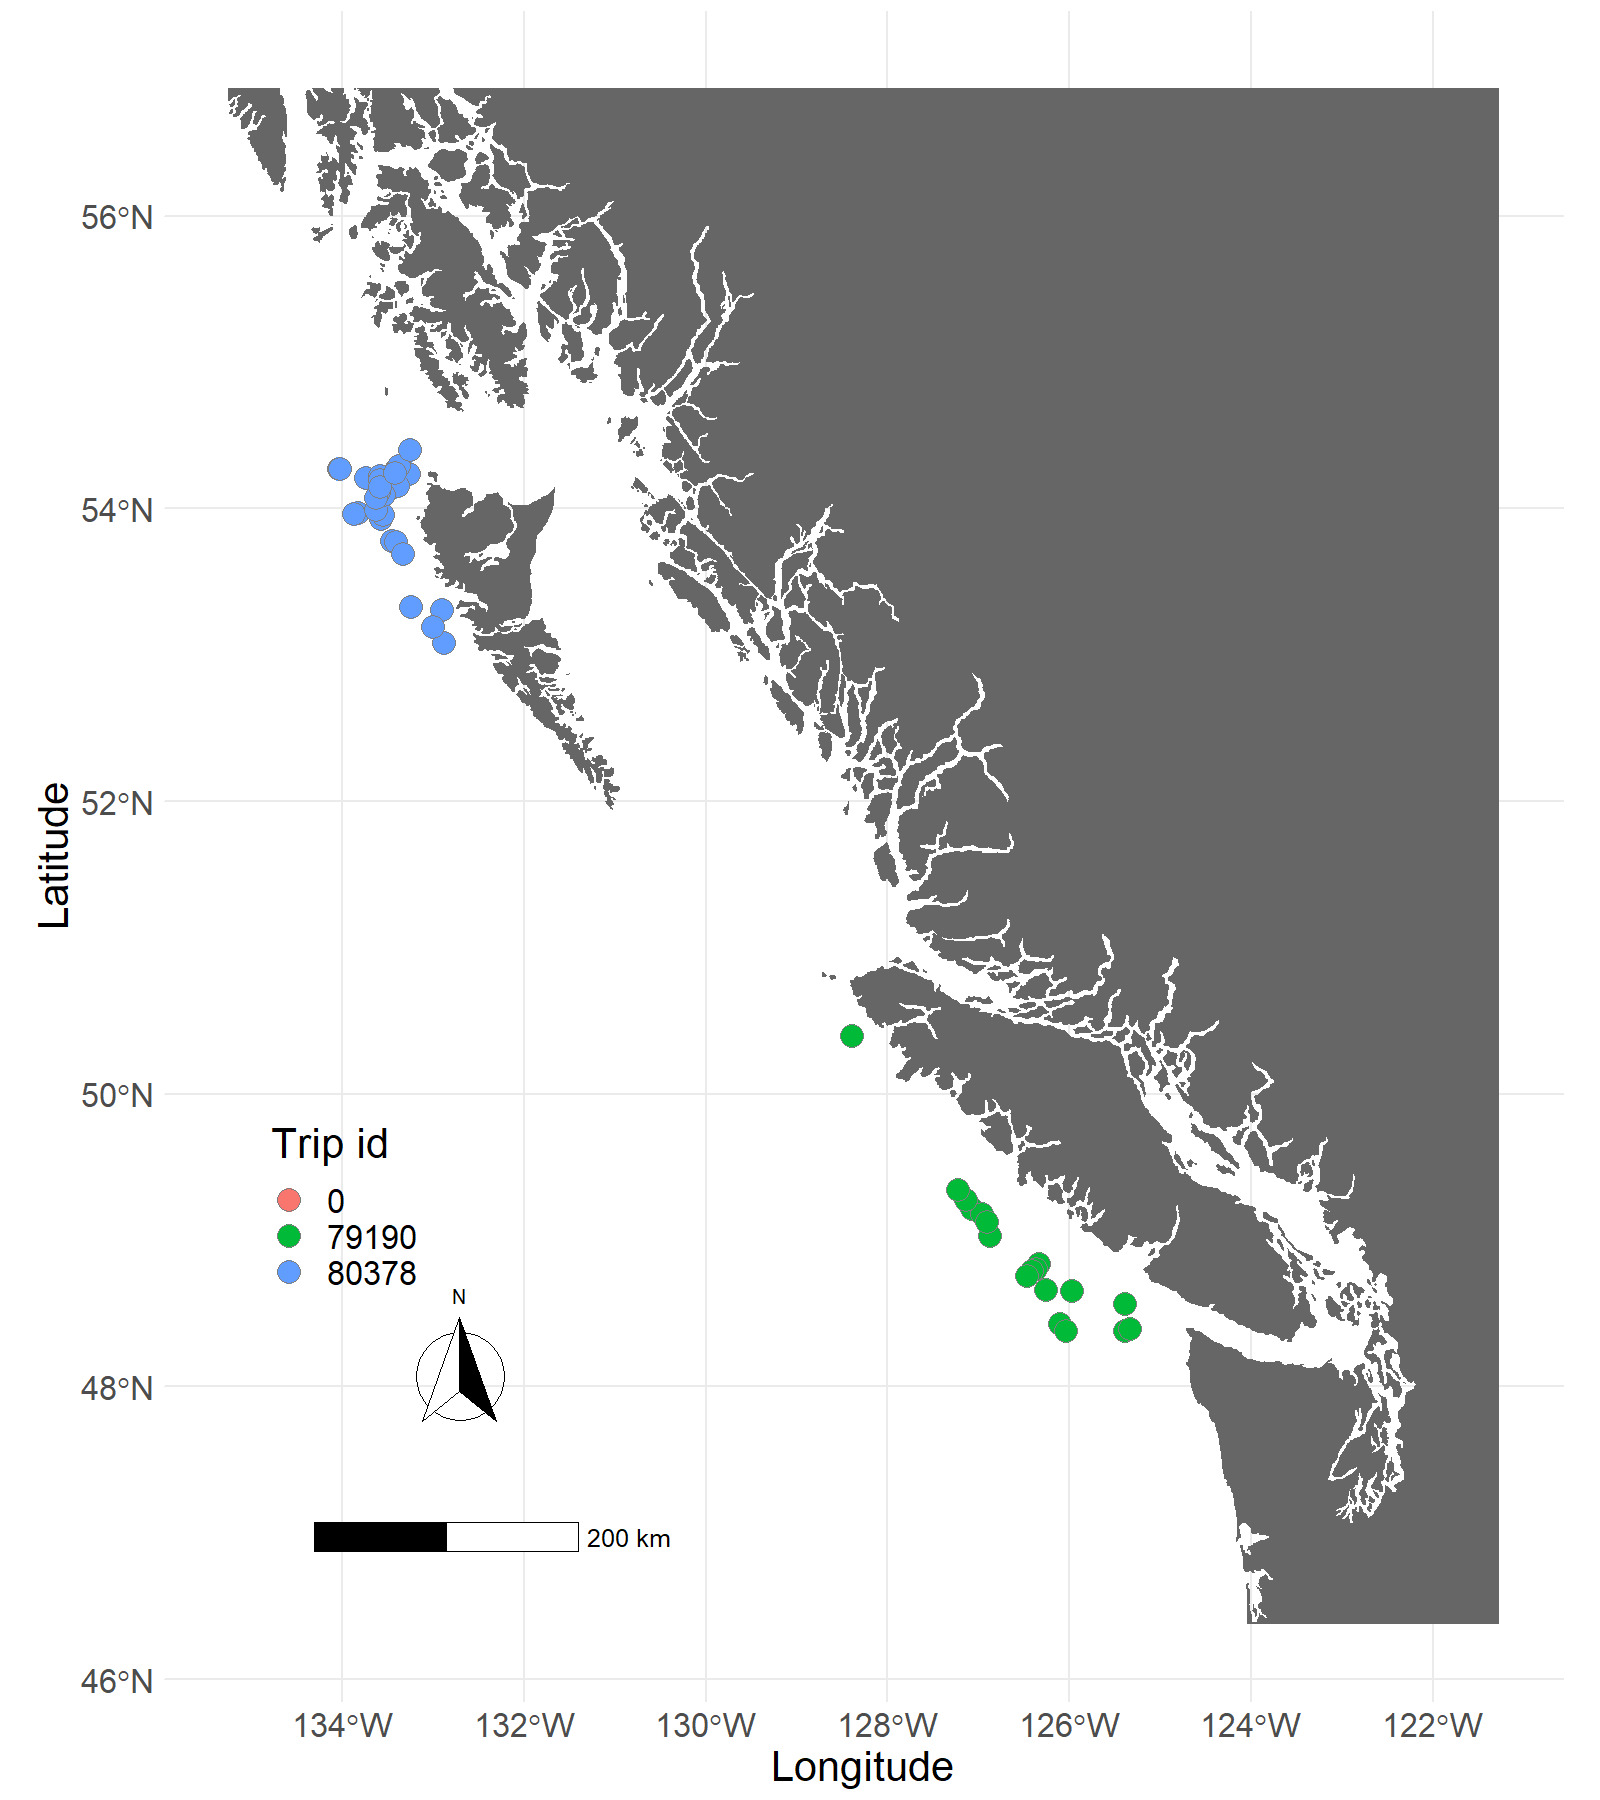
\includegraphics[width=6in]{figures/Figure1}}{Figure} 

}

\caption{Sample locations from the 2016 WCVI, 2016 WCHG research surveys and 2017 pilot study. The sample locations of the salmon survey are unknown.}\label{fig:figure1}
\end{figure}

\begin{figure}[htb]

\pdftooltip{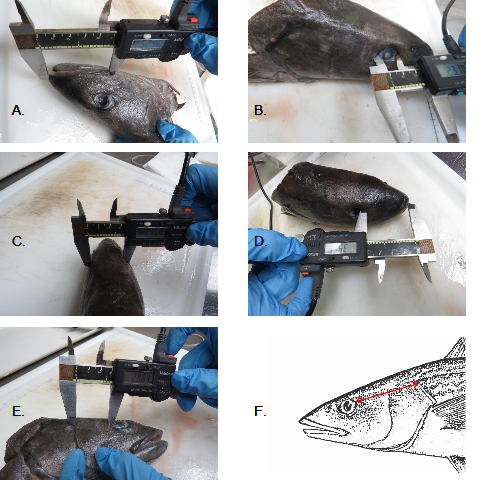
\includegraphics[width=470px]{figures/Figure2}}{Figure} \hfill{}

\caption{Relationship between cranial lengths (UJ-upper jaw, ED-eye diameter, ID-interorbital distance) vs fork length in millimeters. Predicted points represented by black circles, measured values colored by residual scale.}\label{fig:figure2}
\end{figure}

\begin{figure}[htb]

\pdftooltip{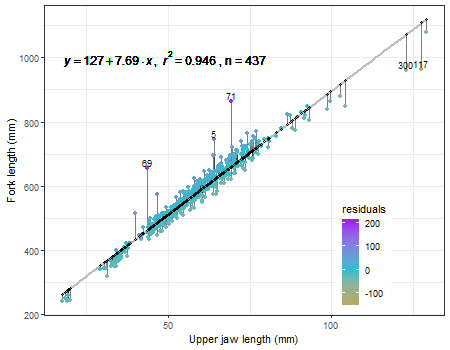
\includegraphics[width=470px]{figures/Figure3}}{Figure} \hfill{}

\caption{Relationship between cranial lengths (SL-snout length, PP-post orbital to preoperculum, PO-post orbital) vs fork length in millimeters. Predicted points represented by black circles, measured values colored by residual scale.}\label{fig:figure3}
\end{figure}

\begin{figure}[htb]

\pdftooltip{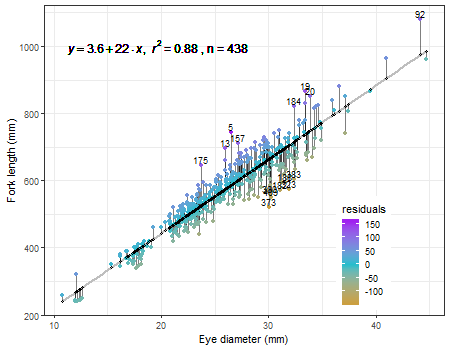
\includegraphics[width=500px]{figures/Figure4}}{Figure} \hfill{}

\caption{Concordance between the science technician sex determinations and the genetics lab results for the 129 successful Sablefish DNA samples. Bubble size indicates the number of specimens and fork length measurements are in mm. Bubbles outlined in red denotes fork length ranges with the lowest concordance.}\label{fig:figure4}
\end{figure}

\begin{figure}[htb]

\pdftooltip{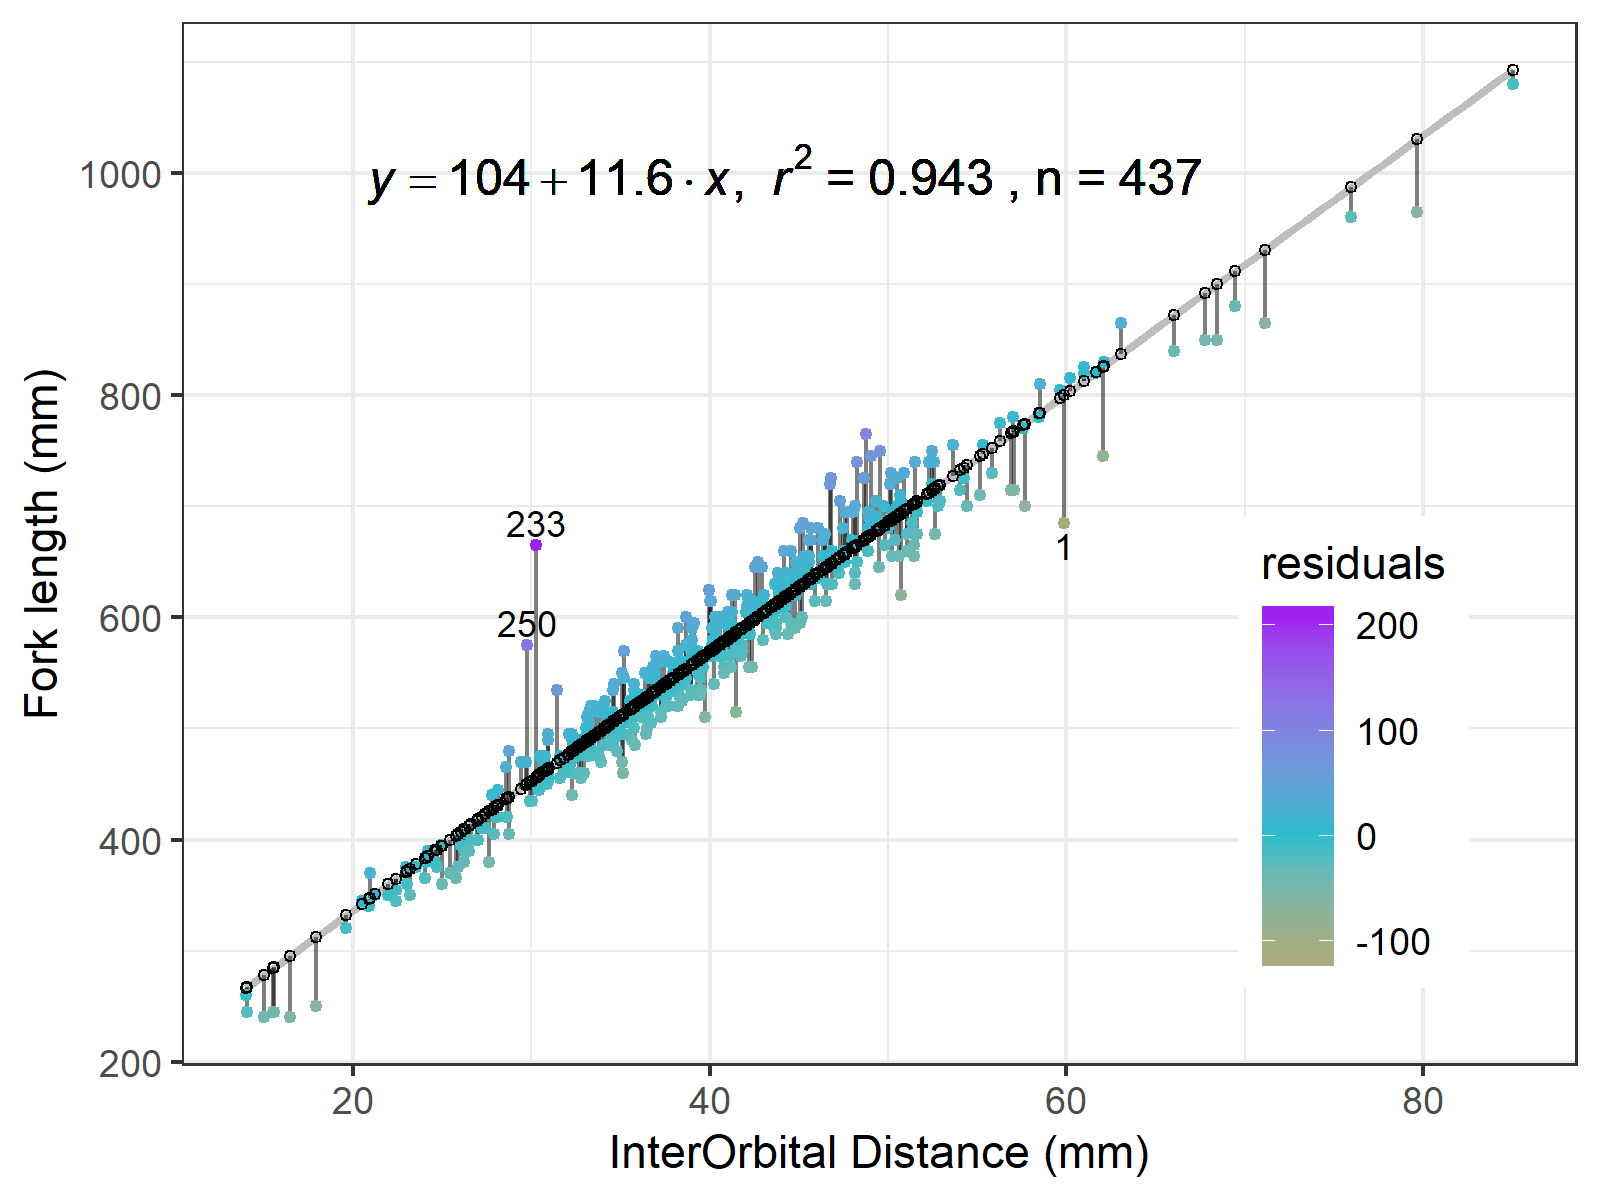
\includegraphics[width=500px]{figures/Figure5}}{Figure} \hfill{}

\caption{Concordance between the fisher sex determinations and the genetics lab results for the 80 successful Sablefish DNA samples. Bubble size indicates number of specimens. Interorbial distance measurements (mm) are presented as average of three measurements. Bubbles outlined in red denotes the average interorbital distance range with the lowest concordance \textgreater{} 1\%.}\label{fig:figure5}
\end{figure}
\clearpage

\hypertarget{tables}{%
\section{Tables}\label{tables}}


\begin{table}[!h]

\caption{\label{tab:table1}List of head dimensions for upper jaw length (L\textsubscript{UJ}), eye diameter (L\textsubscript{ED}), interorbital distance (L\textsubscript{ID}), snout length (L\textsubscript{SL}), post orbital to preoperculum distance (L\textsubscript{PP}) and post orbital head length (L\textsubscript{PO}) measurement descriptions and specification of caliper jaw placement. Many dimensions follow the morphological measurements described in (\protect\hyperlink{ref-Shaw1997}{Shaw and McFarlane 1997}). The matching images for each dimension are found in Appendix A.}
\fontsize{10}{12}\selectfont
\begin{tabular}[t]{>{\raggedright\arraybackslash}p{1.9cm}>{\raggedright\arraybackslash}p{6.0cm}>{\raggedright\arraybackslash}p{7.5cm}}
\toprule
\textbf{Head dimension} & \textbf{Head description} & \textbf{Caliper jaw position}\\
\midrule
L\textsubscript{UJ} & Tip of snout to the posterior edge of the maxilla. & Outside caliper jaw measurement from forward point and centre of snout to back of maxilla.\\
\midrule
L\textsubscript{ED} & Anterior-posterior diameter of eye socket. & Inside caliper jaw measurement firmly stretched against eye socket at vertical midpoint of eye.\\
\midrule
L\textsubscript{ID} & Narrowest distance between eye sockets, measured on dorsal surface. & Outside caliper jaw measurement of the horizontal midpoint of eyes on dorsal surface.\\
\midrule
L\textsubscript{SL} & Tip of snout to anterior inner edge of eye socket. & Outside caliper jaw measurement from forward point and centre of snout to horizontal midpoint of anterior edge of eye socket.\\
\midrule
L\textsubscript{PP} & Posterior inner edge of orbit to visual insertion point of preopercle. & Outside caliper jaw measurement from back of eye socket to preopercle bone insertion point. Preopercle must be lifted to expose preopercle bone underneath.\\
\midrule
L\textsubscript{PO} & Posterior inner edge of orbit to dorsal insertion of opercle. & Outside caliper jaw measurement from back of eye socket to bone underneath gill cover notch at dorsal insertion of the opercle.  The operculum must be held taut.\\
\bottomrule
\end{tabular}
\end{table}
\clearpage


\begin{table}[!h]

\caption{\label{tab:table2}Summary of Sablefish biological data collected during the 2016 experimental study by survey source. Tally of fork lengths (L\textsubscript{FL}), round weights (RW), upper jaw lengths (L\textsubscript{UJ}), eye diameters (L\textsubscript{ED}), interorbital distances (L\textsubscript{ID}), snout lengths (L\textsubscript{SL}), post orbital to preoperculum distances (L\textsubscript{PP}), post orbital head lengths (L\textsubscript{PO}), females (F), males (M), sagittal otoliths and operculum clips (DNA) listed by survey.}
\fontsize{10}{12}\selectfont
\begin{tabular}[t]{lrrrrrrrrrrrrr}
\toprule
\textbf{Survey} & \textbf{L\textsubscript{FL}} & \textbf{RW} & \textbf{L\textsubscript{UJ}} & \textbf{L\textsubscript{ED}} & \textbf{L\textsubscript{ID}} & \textbf{L\textsubscript{SL}} & \textbf{L\textsubscript{PP}} & \textbf{L\textsubscript{PO}} & \textbf{F} & \textbf{M} & \textbf{Otoliths} & \textbf{DNA} & \textbf{Total}\\
\midrule
2016 WCHG & 219 & 219 & 219 & 219 & 218 & 219 & 207 & 52 & 111 & 108 & 219 & 59 & 219\\
2016 WCVI & 212 & 212 & 211 & 212 & 212 & 211 & 212 & 78 & 105 & 107 & 212 & 78 & 212\\
Salmon & 7 & 0 & 7 & 7 & 7 & 7 & 7 & 0 & 0 & 7 & 0 & 0 & 7\\
\midrule
\textbf{Total} & \textbf{438} & \textbf{431} & \textbf{437} & \textbf{438} & \textbf{437} & \textbf{437} & \textbf{426} & \textbf{130} & \textbf{216} & \textbf{222} & \textbf{431} & \textbf{137} & \textbf{438}\\
\bottomrule
\end{tabular}
\end{table}

\begin{table}[!h]

\caption{\label{tab:table3}Model statistics are shown for comparisons of each of the six cranial measurements versus fork length using 438 Sablefish collected from research surveys in 2016. Statistics shown include sample size, Pearson's correlation co-efficients (r), and linear regression statistics for cranial measurements as predictors of fork length, including slope, R-squared values, mean predictor variable, and mean response variable. All measurements are in millimeters. Cranial measurements include: upper jaw length (L\textsubscript{UJ}), eye diameter (L\textsubscript{ED}), interorbital distance (L\textsubscript{ID}), snout length (L\textsubscript{SL}), post orbital to preoperculum length (L\textsubscript{PP}) and post orbital head length (L\textsubscript{PO}). All linear regression models were significant at P \textless0.001.}
\fontsize{10}{12}\selectfont
\begin{tabular}[t]{>{\raggedright\arraybackslash}p{2.2cm}>{\raggedright\arraybackslash}p{1.2cm}>{\raggedleft\arraybackslash}p{0.7cm}>{\raggedleft\arraybackslash}p{0.7cm}>{\raggedleft\arraybackslash}p{0.7cm}>{\raggedleft\arraybackslash}p{0.7cm}>{\raggedleft\arraybackslash}p{0.8cm}>{\raggedleft\arraybackslash}p{0.8cm}>{\raggedleft\arraybackslash}p{0.8cm}>{\raggedleft\arraybackslash}p{0.8cm}>{\raggedright\arraybackslash}p{0.8cm}}
\toprule
\multicolumn{7}{c}{\textbf{ }} & \multicolumn{2}{c}{\textbf{Predictor}} & \multicolumn{2}{c}{\textbf{Response L$_{FL}$}} \\
\cmidrule(l{3pt}r{3pt}){8-9} \cmidrule(l{3pt}r{3pt}){10-11}
\textbf{Cranial Measurement} & \textbf{Sex} & \textbf{N} & \textbf{Slope} & \textbf{SE} & \textbf{R\textsuperscript{2}} & \textbf{r} & \textbf{Mean} & \textbf{SD} & \textbf{Mean} & \textbf{SD}\\
\midrule
L\textsubscript{UJ} & female & 215 & 7.4 & 0.12 & 0.945 & 0.972 & 59.8 & 16.93 & 586.7 & 129.71\\
 & male & 222 & 8.1 & 0.13 & 0.949 & 0.974 & 56.2 & 13.16 & 560.3 & 109.45\\
\midrule
L\textsubscript{ED} & female & 216 & 23.9 & 0.50 & 0.914 & 0.956 & 25.9 & 5.19 & 586.7 & 129.41\\
 & male & 222 & 20.1 & 0.51 & 0.877 & 0.936 & 25.9 & 5.09 & 560.3 & 109.45\\
\midrule
L\textsubscript{ID} & female & 215 & 11.3 & 0.15 & 0.960 & 0.980 & 41.6 & 11.27 & 586.9 & 129.68\\
 & male & 222 & 12.2 & 0.25 & 0.916 & 0.957 & 39.2 & 8.59 & 560.3 & 109.45\\
\midrule
L\textsubscript{SL} & female & 215 & 10.9 & 0.14 & 0.966 & 0.983 & 46.6 & 11.70 & 586.7 & 129.71\\
 & male & 222 & 11.9 & 0.19 & 0.945 & 0.972 & 43.1 & 8.93 & 560.3 & 109.45\\
\midrule
L\textsubscript{PP} & female & 211 & 13.8 & 0.23 & 0.945 & 0.972 & 32.6 & 9.03 & 583.0 & 127.89\\
 & male & 215 & 15.7 & 0.31 & 0.921 & 0.960 & 30.4 & 6.73 & 559.9 & 109.84\\
\midrule
L\textsubscript{PO} & female & 73 & 6.6 & 0.23 & 0.923 & 0.961 & 62.1 & 22.51 & 574.9 & 154.35\\
 & male & 57 & 7.8 & 0.34 & 0.904 & 0.951 & 59.2 & 12.81 & 555.6 & 104.97\\
\bottomrule
\end{tabular}
\end{table}

\begin{table}

\caption{\label{tab:table4}Ease of use and repeatable five point ranking scale recorded by experienced samplers for each cranial measurement for the 2016 experimental study, where 5 = Great; 4 = Good; 3 = Moderate; 2 = Questionable; 1 = Poor.}
\fontsize{10}{12}\selectfont
\begin{tabular}[t]{>{\centering\arraybackslash}p{1.4cm}>{\centering\arraybackslash}p{0.9cm}>{\centering\arraybackslash}p{1.7cm}>{\centering\arraybackslash}p{1.2cm}>{\centering\arraybackslash}p{1.7cm}>{\centering\arraybackslash}p{1.7cm}>{\raggedright\arraybackslash}p{4.6cm}}
\toprule
\multicolumn{1}{c}{\textbf{ }} & \multicolumn{2}{c}{\textbf{5 Point Rank}} & \multicolumn{3}{c}{\textbf{Measurement}} & \multicolumn{1}{c}{\textbf{ }} \\
\cmidrule(l{3pt}r{3pt}){2-3} \cmidrule(l{3pt}r{3pt}){4-6}
\textbf{Head Dimension} & \textbf{Ease of use} & \textbf{Repeatable} & \textbf{Caliper limitation} & \textbf{Bilateral} & \textbf{Bone} & \textbf{Considerations}\\
\midrule
L\textsubscript{UJ} & 3 & 4 & x & x & x & End of the maxilla difficult to define. Caliper jaw position must be in center of snout.\\
\midrule
L\textsubscript{ED} & 3 & 2 &  & x &  & Caliper outside jaw position on soft tissue in eye socket may result in measurement differences.\\
\midrule
L\textsubscript{ID} & 5 & 5 &  &  & x & Tissue is compressed to obtain bone measurement. Easy to determine caliper jaw position.\\
\midrule
L\textsubscript{SL} & 4 & 5 &  & x & x & Caliper jaw position must be in center of snout.\\
\midrule
L\textsubscript{PP} & 4 & 5 &  & x & x & Caliper position on pre-operculum may result in measurement differences.\\
\midrule
L\textsubscript{PO} & 3 & 2 & x & x &  & Operculum damage from handling was observed on several fish.  Endpoints difficult to define. Electronic calipers  malfunctioned with lengths >15 cm.\\
\bottomrule
\end{tabular}
\end{table}

\begin{table}

\caption{\label{tab:table5}Summary of Sablefish biological data collected from the 2017 pilot study to Cobb (n=60) and Eickelberg (n=39) seamounts, measured by three expert technicians using a standardized protocol for the 2017 pilot study. Index of Average Error (IAE) \% values are reported for each of the cranial lengths.}
\fontsize{10}{12}\selectfont
\begin{tabular}[t]{>{\raggedright\arraybackslash}p{1.7cm}>{\raggedleft\arraybackslash}p{2.2cm}>{\raggedleft\arraybackslash}p{2.2cm}>{\raggedleft\arraybackslash}p{2.2cm}>{\raggedleft\arraybackslash}p{1.3cm}}
\toprule
\multicolumn{1}{c}{\textbf{ }} & \multicolumn{1}{c}{\textbf{Sampler A}} & \multicolumn{1}{c}{\textbf{Sampler B}} & \multicolumn{1}{c}{\textbf{Sampler C}} & \multicolumn{1}{c}{\textbf{ }} \\
\cmidrule(l{3pt}r{3pt}){2-2} \cmidrule(l{3pt}r{3pt}){3-3} \cmidrule(l{3pt}r{3pt}){4-4}
\textbf{Head Dimension} & \textbf{Min - Max (mm)} & \textbf{Min - Max (mm)} & \textbf{Min - Max (mm)} & \textbf{IAE}\\
\midrule
L\textsubscript{UJ} & 51.65 - 91.02 & 52.64 - 91.53 & 53.82 - 92.55 & 1.0\\
L\textsubscript{ID} & 35.43 - 61.18 & 35.91 - 60.81 & 34.94 - 60.72 & 1.1\\
L\textsubscript{SL} & 39.67 - 69.27 & 40.38 - 70.37 & 41.03 - 70.32 & 1.2\\
L\textsubscript{PP} & 27.69 - 49.88 & 26.83 - 52.51 & 27.25 - 52.15 & 2.3\\
\bottomrule
\end{tabular}
\end{table}
\clearpage

\begin{appendices}
\counterwithin{figure}{section}
\counterwithin{table}{section}
\counterwithin{equation}{section}

\clearpage

\section{IMAGES OF THE SIX CRANIAL DIMENSION MEASUREMENTS.}
\label{app:first-appendix}

A. Upper jaw measurement (UJ); B. Eye diameter measurement (ED); C. Interorbital distance (ID); D. Snout length (SL); E. Post orbital to preoperculum length measurement (PP); F. Post orbital head length (PO).
\begin{center}\pdftooltip{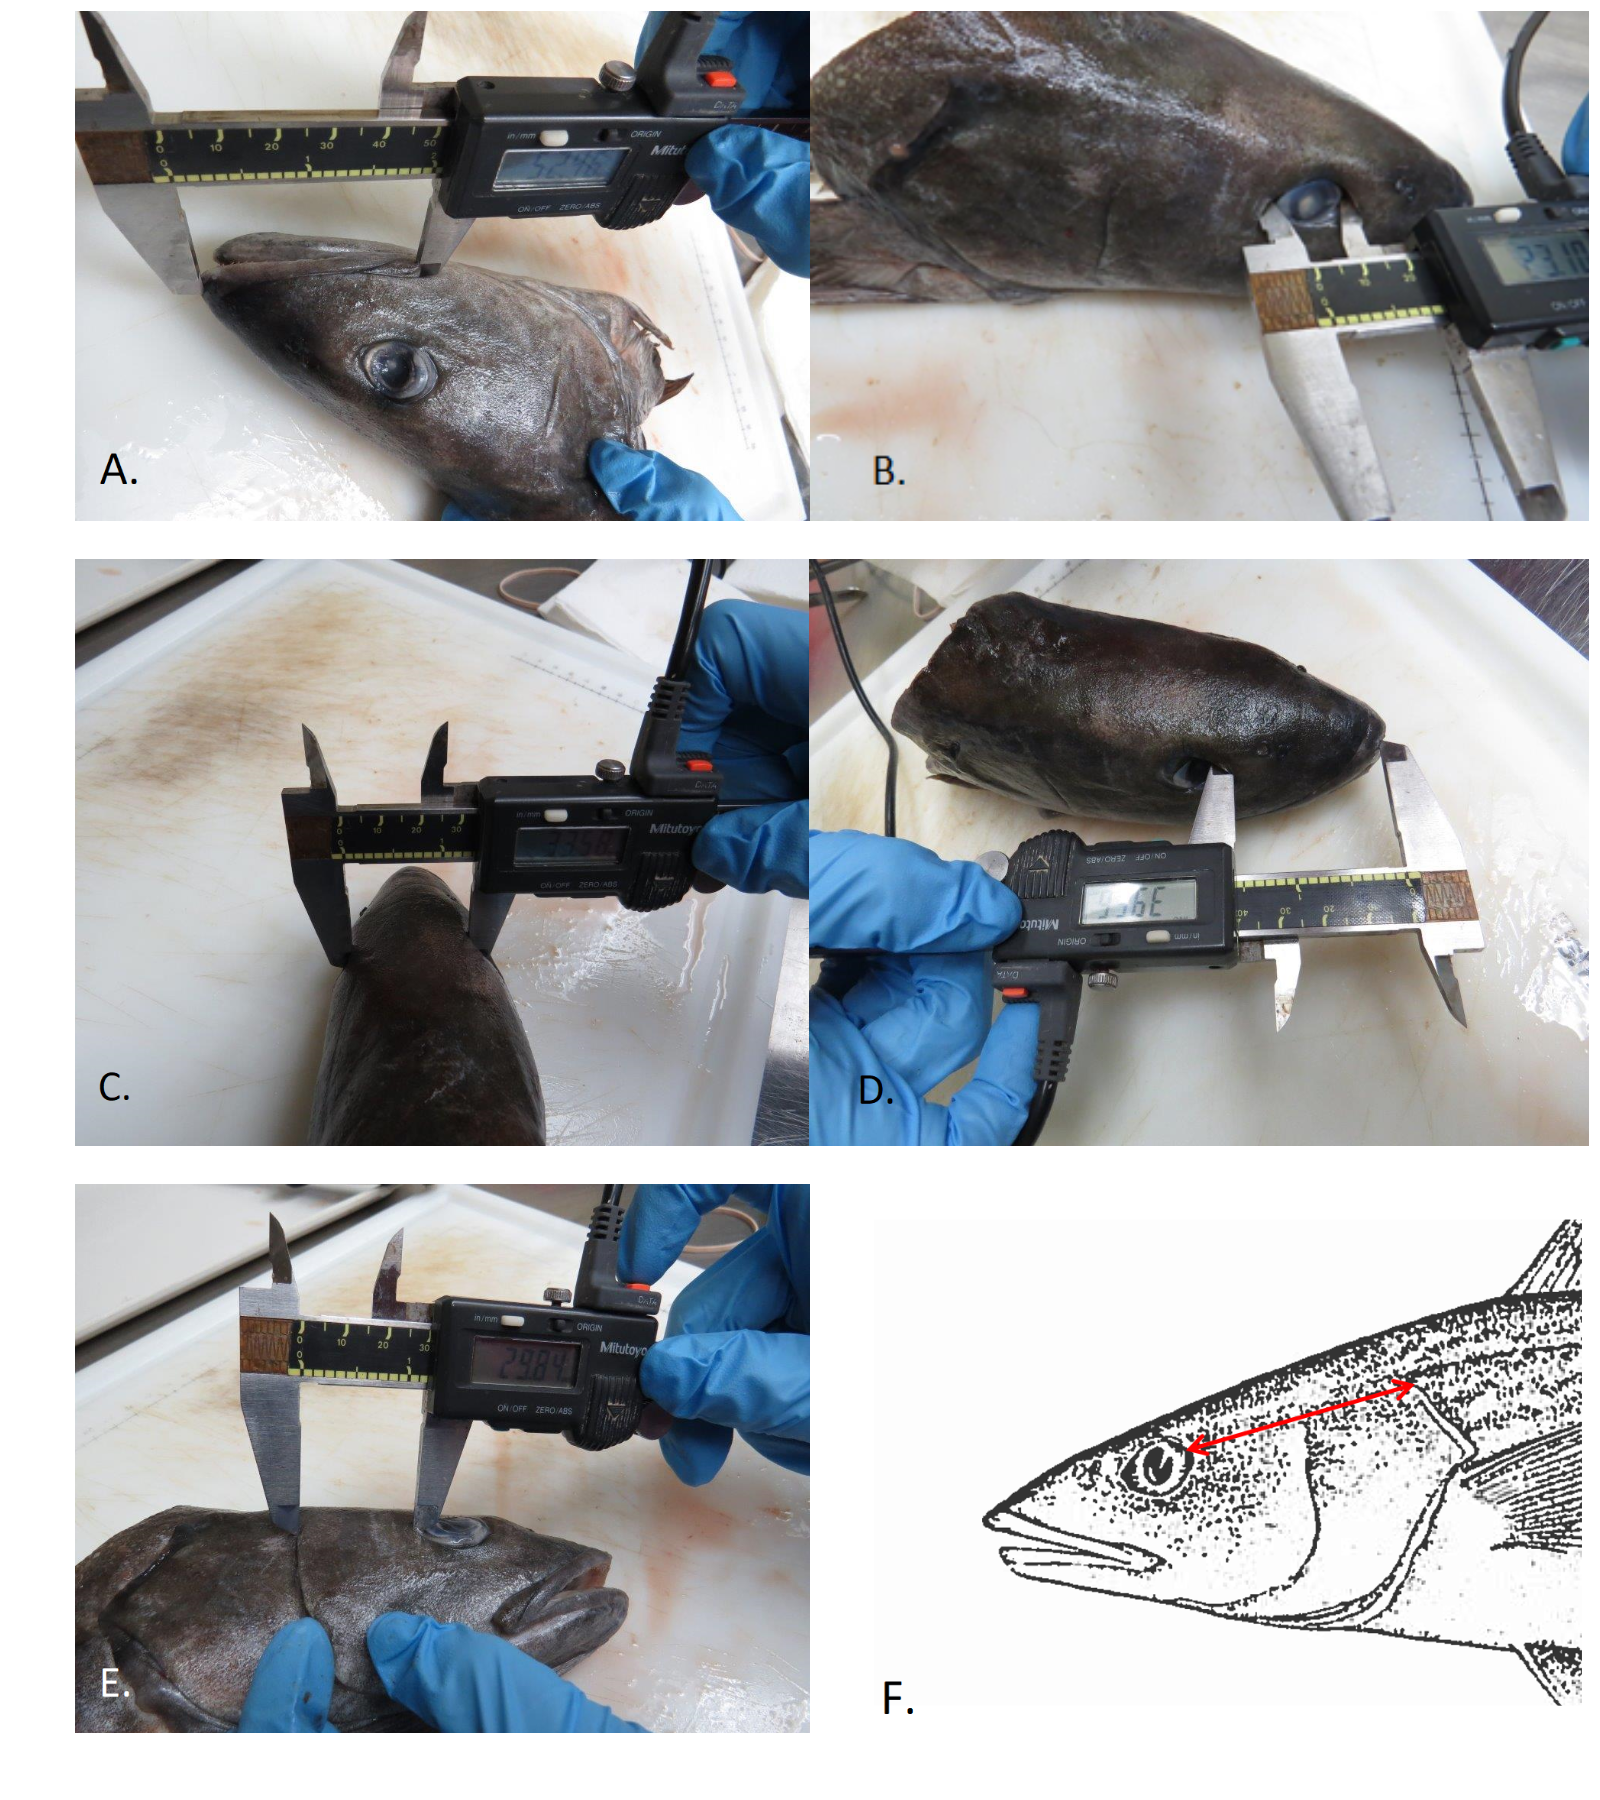
\includegraphics[width=6in]{figures/AppendixA}}{Figure} \end{center}

\clearpage

\section{SEX DETERMINATION BY OPERCULUM MARKING}
\label{app:second-appendix}

Instructions for sex determinations and operculum knife cuts for Sablefish males and females.
\begin{center}\pdftooltip{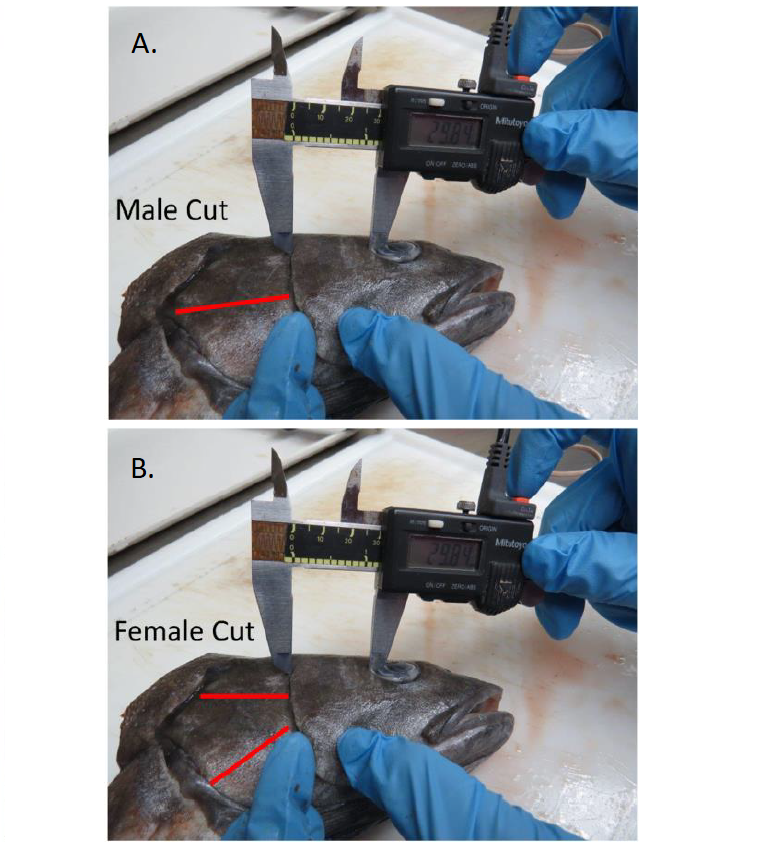
\includegraphics[width=6in]{figures/AppendixB}}{Figure} \end{center}

\section{SABLEFISH BIOSAMPLE COLLECTION PROGRAM NOTICE}
\label{app:third-appendix}

Instructions for the Sablefish biosample collection program.
\begin{center}\pdftooltip{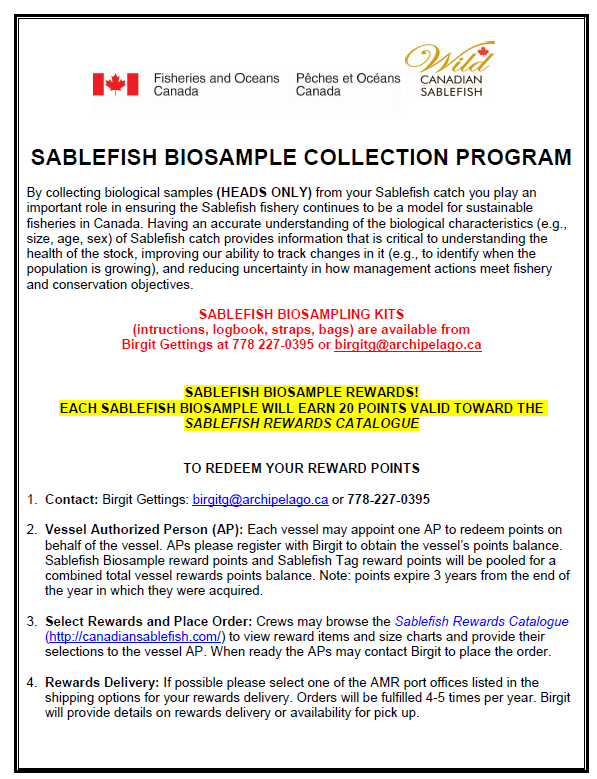
\includegraphics[width=6in]{figures/AppendixC}}{Figure} \end{center}

\section{TAGGED SABLEFISH PROGRAM NOTICE}
\label{app:fourth-appendix}

Instructions for the tagged Sablefish collection program.
\begin{center}\pdftooltip{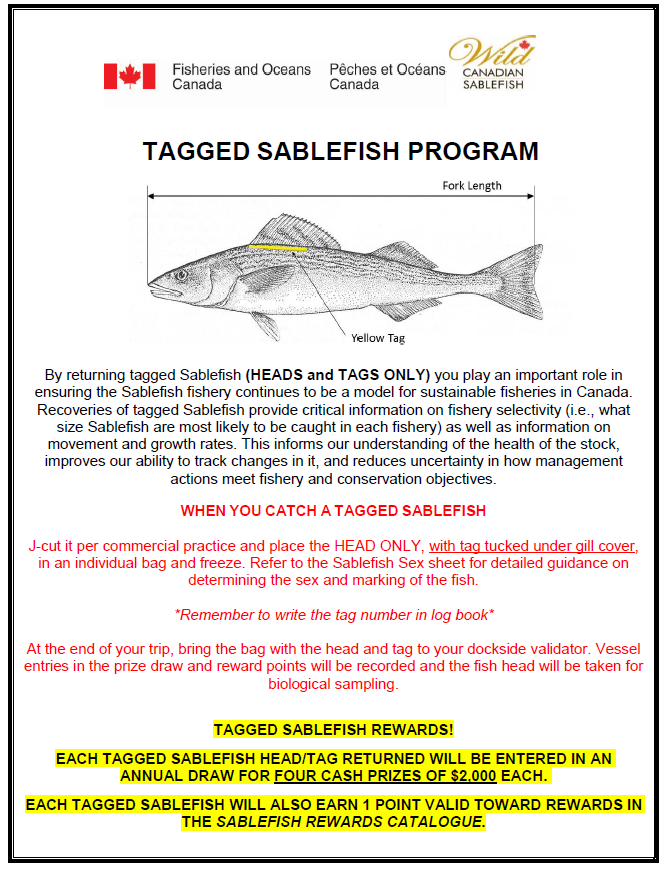
\includegraphics[width=6in]{figures/AppendixD}}{Figure} \end{center}

\clearpage

\end{appendices}

\clearpage

\hypertarget{references}{%
\section{References}\label{references}}

\noindent \vspace{-2em} \setlength{\parindent}{-0.2in} \setlength{\leftskip}{0.2in} \setlength{\parskip}{8pt}

\hypertarget{refs}{}
\begin{CSLReferences}{1}{0}
\leavevmode{\hypertarget{ref-Beamish1981}{}}%
Beamish, R., and Fournier, D.D.A. 1981. \link{https://doi.org/10.1139/f81-132}{A {M}ethod for {C}omparing the {P}recision of a {S}et of {A}ge {D}eterminations}. Canadian Journal of Fisheries and Aquatic Sciences 38: 982--983.

\leavevmode{\hypertarget{ref-Cox2019}{}}%
Cox, S.P., Holt, K., and Johnson, S. 2019. \link{https://waves-vagues.dfo-mpo.gc.ca/library-bibliotheque/40853330.pdf}{Evaluating the robustness of management procedures for the {Sablefish} ({\emph{Anoplopoma fimbria}}) fishery in {British Columbia, Canada} for 2017-18.} DFO Can. Sci. Advis. Sec. Res. Doc. 2019/032. vi + 79 p.

\leavevmode{\hypertarget{ref-Cox2023}{}}%
Cox, S.P., Kronlund, A.R., Lacko, L., and Jones, M. 2023. \link{https://waves-vagues.dfo-mpo.gc.ca/library-bibliotheque/41110961.pdf}{A {R}evised {O}perating {M}odel for {S}ablefish in {B}ritish {C}olumbia, {C}anada in 2016.} DFO Can. Sci. Advis. Sec. Res. Doc. 2023/023. vii + 127 p.

\leavevmode{\hypertarget{ref-Haist2001}{}}%
Haist, R.H., V., and Wyeth, M. 2001. \link{https://publications.gc.ca/collections/collection_2015/mpo-dfo/Fs70-5-2001-135-eng.pdf}{Sablefish {Stock Assessment} for 2001 and {Advice to Managers} for 2002.} DFO Can. Sci. Advis. Sec. Res. Doc. 2001/135.

\leavevmode{\hypertarget{ref-Isermann2005}{}}%
Isermann, D.A., and Vandergoot, C.S. 2005. \link{https://doi.org/10.1577/M04-010.1}{Predicting {W}alleye {T}otal {L}ength from {H}ead and {M}andible {M}easurements}. North American Journal of Fisheries Management 25(1): 316--321. Taylor \& Francis.

\leavevmode{\hypertarget{ref-Nottingham2018}{}}%
Nottingham, M.K., Williams, D.C., Wyeth, M.R., and Olsen, N. 2018. \link{https://waves-vagues.dfo-mpo.gc.ca/library-bibliotheque/40757791.pdf}{Summary of the {West Coast Haida Gwaii Synoptic Bottom Trawl} {S}urvey, {A}ugust 25 - {S}eptember 26, 2016.} Can. Manuscr. Rep. Fish. Aquat. Sci. 3151: viii: 51 p.

\leavevmode{\hypertarget{ref-Park2007}{}}%
Park, I.S., Kim, Y.J., Choi, H.J., Oh, S.Y., Noh, C.H., and Lee, S.H. 2007. \link{https://koreascience.kr/article/JAKO200710103466881.pdf}{Total {L}ength {E}stimation from {H}ead {D}imensions of {A}rtificially {P}ropagated {B}rown {C}roaker {\emph{Miichthys miiuy}}}. Korean J. Ichthyol. 19: 128--131.

\leavevmode{\hypertarget{ref-R}{}}%
R Core Team. 2021. \link{https://www.R-project.org}{R: {A} {L}anguage and {E}nvironment for {S}tatistical {C}omputing}. R Foundation for Statistical Computing, Vienna, Austria.

\leavevmode{\hypertarget{ref-Richardson2015}{}}%
Richardson, J., Shears, N., and Taylor, R. 2015. \link{https://doi.org/10.3354/meps11476}{Using relative eye size to estimate the length of fish from a single camera image}. Marine Ecology Progress Series 538.

\leavevmode{\hypertarget{ref-Rondeau2013}{}}%
Rondeau, E.B., Messmer, A.M., Sanderson, D.S., Jantzen, S.G., Schalburg, K.R. von, Minkley, D.R., Leong, J.S., Macdonald, G.M., Davidsen, A.E., Parker, W.A., Mazzola, R.S.A., Campbell, B., and Koop, B.F. 2013. \link{https://doi.org/10.1186/1471-2164-14-452}{Genomics of {S}ablefish ({\emph{Anoplopoma fimbria}}: Expressed genes, mitochondrial phylogeny, linkage map and identification of a putative sex gene}. BMC Genomics 14(1): 452. Journal Article.

\leavevmode{\hypertarget{ref-Serafy1996}{}}%
Serafy, J.E., Schmitz, C.M., Capo, T.R., Clarke, M.E., and Ault, J.S. 1996. \link{https://doi.org/10.1577/1548-8640(1996)058\%3C0289:TLEORD\%3E2.3.CO;2}{{T}otal {L}ength {E}stimation of {R}ed {D}rum from {H}ead {D}imensions}. The Progressive Fish-Culturist 58(4): 289--290. Taylor \& Francis.

\leavevmode{\hypertarget{ref-Shaw1997}{}}%
Shaw, W., and McFarlane, G. 1997. \link{https://www.researchgate.net/publication/285860984_Development_of_sablefish_Anoplopoma_fimbira_larvae_off_the_West_Coast_of_British_Columbia_and_transformation_in_the_juvenile_stage}{Development of {S}ablefish, {\emph{Anoplopoma fimbria}} larvae off the {W}est {C}oast of {B}ritish {C}olumbia and transformation in the juvenile stage}. NOAA Tech. Rep. NMFS 130: 3--12.

\leavevmode{\hypertarget{ref-Williams2018}{}}%
Williams, D.C., Nottingham, M.K., Olsen, N., and Wyeth, M.R. 2018. \link{https://waves-vagues.dfo-mpo.gc.ca/library-bibliotheque/4075781x.pdf}{Summary of the {West Coast Vancouver Island Synoptic Bottom Trawl} {S}urvey, {M}ay 24 - {J}une 15, 2016.} Can. Manuscr. Rep. Fish. Aquat. Sci. 3137: viii: 54 p.

\end{CSLReferences}
\end{document}
